\documentclass[pageno]{jpaper}

%replace XXX with the submission number you are given from the ASPLOS submission site.
\newcommand{\asplossubmissionnumber}{14}

\usepackage[normalem]{ulem}
\usepackage{appendix}
\usepackage{amsmath}

\DeclareMathOperator*{\argmax}{argmax}
\DeclareMathOperator*{\argmin}{argmin}

\begin{document}

\title{
Compiling Physical Invariants to Hardware for a Secure \& Private Sensor Interface}

\date{December 2018}
\maketitle

\thispagestyle{empty}

\begin{abstract}

The aim of this report is to outline the progress made so far with this project, as well as detail the strategy that will lead to completion of the remaining work within the remaining time. Firstly, the project aims and motivation will be described, as the initial project specification has evolved over time to reach its current state (from simply compiling information about physical invariants into HDL to implementing a local differential privacy system that uses this information to account for the mutual privacy loss between related electronic sensors). Next, the most recent proposal for a multi sensor differential privacy system will be detailed, including description and analysis of prototying work in Python and Verilog. Finally, the project timetable will be presented, outlining and justifying remaining tasks and allocated timeframes.

\end{abstract}

\section{Introduction}
\subsection{Background}

The project is based on the Newton description language, designed by Jonathan Lim and Phillip Stanley-Marbell\cite{Newton}. The language provides a way of describing relationships between physical properties e.g. those measured by electronic sensors in an embedded computing system. The starting point for this project was to investigate applications of compiling Newton descriptions into a hardware description language such as Verilog, which could then be synthesised into hardware on a low power iCE40\cite{iCE40} FPGA.

\begin{figure}[h]
  \centering
    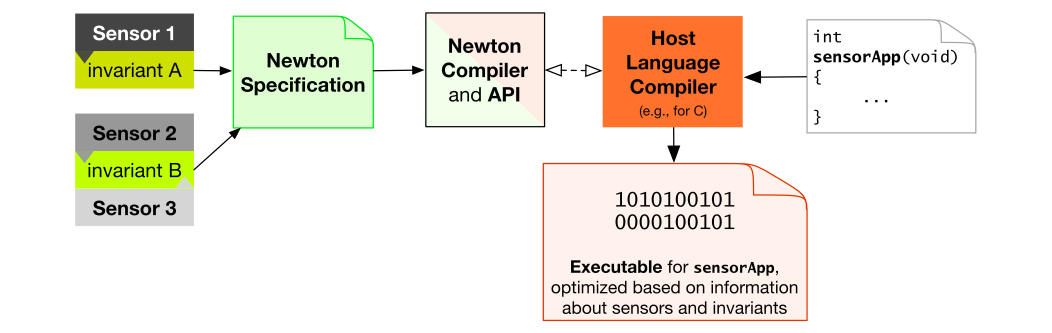
\includegraphics[width=\columnwidth]{images/Newton-and-C-Compiler-Interaction.png}
    \caption{\textit{The Newton language was initially designed to be used with an API called by a host language compiler\cite{Newton}. For this project, the host language 'compiler' will be a custom C program that uses information from a Newton description to modify an existing Verilog template.}}
    \label{fig:newton_compiler_interaction}
\end{figure}

The existing Newton compiler 'frontend' is a C/C++ program that parses a description in the Newton language, arranging information into an abstract syntax tree. This project focuses on a compiler 'backend', a C/C++ program that uses the information in this tree to, in this case, generate Verilog to configure an iCE40 FPGA.

\subsection{Project Aims and Motivation}
Simply compiling a Newton description into a hardware description language is not a useful research topic as it does not provide any particular insight, nor do anything particularly new. With this in mind, a new motivation for the project was conceived, with the aim of investigating a practical application of Newton within a data security and privacy context. Specifically, this project aims to investigate the idea of utilising information from a Newton description in a multi-sensor local differential privacy system (an embedded system consisting of electronic sensors and an iCE40 FPGA acting as the interface to the outside world) in order to be able to account for the mutual information between sensor measurements. This differential privacy system would aim to mask the true value of sensor measurements whilst still providing some useful information by adding zero mean random noise. Unlike existing work regarding local differential privacy systems involving a single sensor/value to be masked\cite{Choi2018GuaranteeingLD}, a system with multiple related sensors must be able to account for the information an attacker can gain about one measurement by taking related measurements e.g. inferring velocity from position measurements.

\subsection{Review of Existing Work}
At the start of the project, it was important to review existing work in order to determine the current state of the art and to discover useful ideas and techniques that could be incorporated into this project. Examples of reviewed publications include:
\begin{itemize}
\item \textbf{"Guaranteeing Local Differential Privacy
on Ultra-low-power Systems"} - \textit{Woo-Seok Choi, Matthew Tomei, Jose Rodrigo Sanchez Vicarte, Pavan Kumar Hanumolu, Rakesh Kumar.}\cite{Choi2018GuaranteeingLD}\\
This paper analyses the feasibility of implementing a local differential privacy system on low power fixed point hardware (such as an iCE40 FPGA). It suggests solutions to privacy loss problems caused by the finite (and relatively constrained) precision with which numerical values are represented on such hardware. The 'DP-box' architecture described in the paper provided a detailed foundation for the architecture of this system.
\item \textbf{"A Hardware Efficient Random Number Generator for
NonuniformDistributions with Arbitrary Precision"} - \textit{Christian de Schryver, Daniel Schmidt, NorbertWehn, Elke Korn,
HenningMarxen, Anton Kostiuk and Ralf Korn}\cite{DeSchryver}\\
This paper describes a hardware efficient (i.e. uses relatively few LUTs in an FPGA) method for generating random samples from an arbitrary distribution, based on the inversion method. It describes a hardware system for representing a uniform random bit vector in floating point form, using the exponent and mantissa as the address input to a lookup table. This allows for efficient estimation of the inverse cumulative distribution function (ICDF) for an arbitrary probability distribution via linear interpolation.
\item \textbf{"FPGA-Based True Random Number Generation Using Circuit Metastability with Adaptive Feedback Control"} - \textit{Mehrdad Majzoobi, Farinaz Koushanfar
and Srinivas Devadas}\cite{trng}\\
One important component of the project is a 'true' random number generator (TRNG) - a pseudorandom number generator is insufficient for a security application where an attacker must not be able to predict the random output. This paper illustrates one method of providing randomness by clocking a D flip flop whilst changing the state of the input during the setup/hold time (metastable region) so that the flip flop output is non-deterministic. Additional proportional \& integral feedback control logic is suggested as a method for minimising bias in the output, with control being implemented via single LUT programmable delay lines. One other TRNG implementation to be investigated involves sampling from the iCE40 device's differential I/O pins, effectively using two pins as a comparator with floating inputs. This could potentially result in simpler logic circuitry compared to the approach described in this paper.
\end{itemize}

\section{System Description}
The following section aims to describe the planned architecture for the FPGA based system being developed. The Lattice iCE40 FPGA has been selected for its small size, low cost and low power consumption - in theory, it could be incorporated into the package of future electronic sensors. The FPGA acts as an interface between electronic sensors and external circuitry e.g. a microprocessor. External circuitry will be able to query the FPGA for a measurement from a particular sensor; the FPGA responds by taking a measurement and adding zero mean Laplace distributed noise in order to mask the true value of the measurement (local differential privacy). This process has revealed information about the true value being measured, so the FPGA must also maintain a privacy 'budget' for each sensor. Responding to a query results in a privacy loss i.e. deduction from the relevant privacy budget, both for the sensor being queried and also for related sensors - for example, measuring GPS position against time reveals information about a device's velocity, so the system must be able to deduct from the privacy budgets for both position and velocity when responding to position queries. The FPGA therefore requires information about the relationships between sensors in the system - this is provided by a Newton description, compiled into Verilog by a C program (the 'compiler' section of the project). A detailed description of the planned system for multi-sensor privacy budget management is given in section \ref{subsection:multi_sensor}.

\section{Michaelmas Term Progress}
Project source code can be found on GitHub at https://github.com/Gregox273/Newton-Verilog-Compiler/. This includes Python prototyping code as well as Verilog and the Newton to Verilog compiler (written in C).

\subsection{Preparation and Background Reading}
As mentioned above, an important step at the start of the project was to read through existing literature in order to decide upon a new research topic to investigate, as well as gather useful information and techniques to build upon. This process was facilitated by attending weekly meetings with the Physical Computation\cite{physcomp} research group, where papers were read, analysed, discussed and summarised by the group.

\subsection{Extending Differential Privacy to Multi-Sensor Systems} \label{subsection:multi_sensor}
Some progress has been made regarding the mathematics behind a multi-sensor differential privacy system, specifically the effect that responding to a query !!!!!!!!!!!!!!!!!!!!!!!!!!!!!!!!!!!!!!!!!!!!!!!!!!!!!!!!!!!!!!!!!!!!!

A \ref{appendix:upper_bound}!!!!!!!!!!!!!!!!!!!!!!!!!!!!!!!!!!!!!. From this result we can conclude that for some relationship between N measurements:
\begin{itemize}
  \item If fewer than N-1 measurements have been taken, then no information has been gained about the remaining (unmeasured) variables
  \item If one more measurement is taken (N-1 measurements have been taken) then the final unmeasured value can be calculated from these 'known' i.e. measured values. The privacy loss experienced by the 'unknown' value is bounded by the sum of privacy losses incurred by the N-1 measurements that have been taken.
  \item Each subsequent measurement of one of the N-1 'known' quantities will result in additional indirect privacy loss in the 'unknown' value, bounded by the direct privacy loss experienced by the 'known' quantity.
\end{itemize}

\subsection{Prototying}
It was decided that prototyping the differential privacy system in a high level scripting language such as Python would allow for rapid testing, debugging and evaluation of proposed system architectures, algorithms, data representations etc.. To date, the Python simulation contains an implementation of the floating point random number generator architecture described above\cite{DeSchryver}, as well as class definitions to represent hardware sensors, sensor interfaces, and relationships between quantities present in a Newton description.

\subsection{Verilog}
Most of the time allocated to this part of the project has been spent getting acquainted with the Verilog language - so far, synthesisable modules have been generated to implement logic converting a uniform random bit vector to a floating point representation (as described by De Schryver et al.\cite{DeSchryver}), including logic to count leading zeros in a bit vector. Care has been taken to ensure the Verilog hardware descriptions are flexible and easily reconfigurable e.g. variable bit widths for registers and module I/O wires, with useful constants being defined in header files that can be written manually or generated by a script/program such as the compiler portion of the project. A lookup table approximating the inverse cumulative distribution function for the Laplace distribution has also been implemented, with table contents being taken from an external autogenerated file.

\subsection{Newton to Verilog Compiler}
The overall aim of the project is to produce a Newton compiler 'backend' written in C/C++. Initial steps have been taken to build up this body of code in a modular and flexible way. Currently, the C program is able to generate Verilog header files defining useful constants, reading data in from a YAML file. In future, the contents of this YAML file will be expanded to include differential privacy related information such as the privacy budget and budget refresh rate for each sensor in the system. The program also generates the fixed point lookup table entries required for the FPGA to be able to efficiently estimate the ICDF for a Laplace (or potentially any other) distribution.

\section{Project Timetable}
\subsection{Summary of Completed Work}
\subsection{Timetable}
\subsection{Justification for Changes}

\begin{appendices}
\section{Upper Bound on Indirect Privacy Loss}
\label{appendix:upper_bound}
Let y be a value derived from sensor measurements $x_i$:
\begin{equation} \label{eqn:ub_y}
  y = f_y(x_1, x_2,..., x_n) = f_y(\mathbf{x})
\end{equation}
\\
Noised sensor outputs $X_i$ are generated by adding random noise $n_i$ to sensor measurements:
\begin{equation} \label{eqn:ub_X_i}
  X_i = x_i + n_i
\end{equation}
\\
This results in a noised value for the inferred quantity:
\begin{equation} \label{eqn:ub_Y}
  Y = f_y(X_1, X_2,..., X_n) = f_y(\mathbf{X})
\end{equation}
\\
The maximum privacy loss resulting from a response to a query is given by\cite{Choi2018GuaranteeingLD}:
\begin{equation} \label{eqn:ub_l_y}
  l_y = log\left( \frac{p(Y|y_i)}{p(Y|y_j)} \right)
\end{equation}
for $y_i, y_j = \argmax_{y_i, y_j} l_y(y_i, y_j)$
\\\\
This can be rewritten in the form:
\begin{equation} \label{eqn:ub_l_y_2}
  l_y = log\left( \frac{p(\mathbf{X}|y_i)}{p(\mathbf{X}|y_j)} \right) \nonumber
\end{equation}
\begin{equation} \label{eqn:ub_l_y_constrained}
  l_y = log\left( \frac{p(\mathbf{X}|\mathbf{x}_i)}{p(\mathbf{X}|\mathbf{x}_j)} \right)
\end{equation}
where $\mathbf{x}_i = \argmax_{\mathbf{x}_i} f_y(\mathbf{x}_i)$ and $\mathbf{x}_j = \argmin_{\mathbf{x}_j} f_y(\mathbf{x}_j)$
\\\\
This constrained optimisation problem can be directly solved to find a value for privacy loss e.g. via Lagrange multipliers. However, a simpler calculation can be performed to provide an upper bound on privacy loss by removing the constraints on $\mathbf{x}_i, \mathbf{x}_i$:
% \begin{equation} \label{eqn:ub_l_y_unconstrained}
%   l_y = log\left( \frac{max(p(\mathbf{X}|\mathbf{x}_i))}{min(p(\mathbf{X}|\mathbf{x}_j))} \right) \nonumber
% \end{equation}
\begin{equation} \label{eqn:ub_l_y_expanded}
  l_y = log\left( \frac{max[p(X_1 | x_{1i})p(X_2 | x_{2i})...p(X_n | x_{ni})]}{min[p(X_1 | x_{1j})p(X_2 | x_{2j})...p(X_n | x_{nj})]} \right) \nonumber
\end{equation}
\begin{equation} \label{eqn:ub_l_y_unconstrained}
  l_y \leq log\left( \prod_{u=1}^n \frac{max[p(X_u|x_{ui})]}{min[p(X_u|x_{uj})]} \right)
\end{equation}
\\
This upper bound on privacy loss is equal to the sum of privacy losses deducted from the budgets of measurements $x_1$ to $x_n$.
\end{appendices}

% %%%%%%%%%%%%%%%%%%%%%%%%%%%%%%%%%%%%%%%%%%%%%%%%%%%%%%%%%%%%%%%%%%%%%%
% \clearpage
% \section{Introduction}
%
% % This document provides instructions for submitting papers to the 23rd
% % International Conference on Architectural Support for Programming
% % Languages and Operating Systems (ASPLOS), 2018.  In an effort to
% % respect the efforts of reviewers and in the interest of fairness to
% % all prospective authors, we request that all submissions to ASPLOS
% % 2018 follow the formatting and submission rules detailed below.
% % Submissions that violate these instructions may not be reviewd, at the
% % discretion of the program chair, in order to maintain a review process
% % that is fair to all potential authors.
% %
% % An example submission (formatted using the ASPLOS'18 submission
% % format) that contains the submission and formatting guidelines can be
% % downloaded from here:
% % \href{https://www.asplos2018.org/wp-content/uploads/2017/07/asplos18-template.pdf}{Sample PDF}. The content of
% % this document mirrors that of the submission instructions that appear
% % on \href{https://www.asplos2018.org/submissions/}{this
% % website}, where the paper submission site will be linked online
% % shortly.
% %
% % All questions regarding paper formatting and submission should be directed
% % to the program chair.
%
% \paragraph{Highlights ({\bf note the following})}:
% \begin{itemize}
% \item Paper must be submitted in printable PDF format.
% \item Text must be in a minimum 10pt ({\bf not} 9pt) font.
% \item Papers must be submitted in printable PDF format and should contain a
% maximum of 11 pages of single-spaced two-column text, including any
% appendixes, but not including references.
% \item No page limit for references.
% \item Each reference must specify {\em all} authors (no {\em et al.}).
% \item Authors may optionally suggest reviewers.
% \item Authors of {\em all} accepted papers will be required to give a
% lightning presentation (about 90s) and a poster in addition to the regular
% conference talk.
% \item Proceedings will appear in the ACM digital library up to two weeks
% before the conference.
% \end{itemize}
%
% \paragraph{Paper evaluation objectives}:
%
% The committee will make every effort to judge each submitted paper on
% its own merits. There will be no target acceptance rate.  We expect to
% accept a wide range of papers with appropriate expectations for
% evaluation --- while papers that build on significant past work with
% strong evaluations are valuable, papers that open new areas with less
% rigorous evaluation are equally welcome and especially encouraged.
% Given the wide range of topics covered by ASPLOS, every effort will be
% made to find expert reviewers, including providing the ability for
% authors' to suggest additional reviewers.
% \section{Paper Preparation Instructions}
%
% \subsection{Paper Formatting}
%
% Papers must be submitted in printable PDF format and should contain a
% {\bf maximum of 11 pages} of single-spaced two-column text, including any
% appendixes, but {\bf not
%   including references}.  You may include any number of pages for
% references, but see below for more instructions.  If you are using
% \LaTeX~\cite{lamport94} to typeset your paper, then we suggest that
% you use the template here:
% \href{https://www.asplos2018.org/wp-content/uploads/2017/07/asplos18-latex-template.tar.gz}{\LaTeX~Template}.
% (\href{https://www.asplos2018.org/wp-content/uploads/2017/07/asplos18-template.pdf}{This
%   document} was prepared with that template.)  If you use a different
% software package to typeset your paper, then please adhere to the
% guidelines given in Table~\ref{table:formatting}.\footnote{One
%   exception is that authors may use the SIGPLAN style/class file
%   \href{http://classic.sigplan.org/sigplanconf.cls}{here}, but {\bf
%     only with the 10pt body font option (9pt will be rejected)} and
%   modified as needed for the requirements of the references section
%   below.  This is marginally different from the specified template,
%   but will be accepted due to its widespread use.}
%
% \begin{table}[h!]
%   \centering
%   \begin{tabular}{|l|l|}
%     \hline
%     \textbf{Field} & \textbf{Value}\\
%     \hline
%     \hline
%     File format & PDF \\
%     \hline
%     Page limit & 11 pages, {\bf not including}\\
%                & {\bf references}\\
%     \hline
%     Paper size & US Letter 8.5in $\times$ 11in\\
%     \hline
%     Top margin & 1in\\
%     \hline
%     Bottom margin & 1in\\
%     \hline
%     Left margin & 0.75in\\
%     \hline
%     Right margin & 0.75in\\
%     \hline
%     Body & 2-column, single-spaced\\
%     \hline
%     Separation between columns & 0.25in\\
%     \hline
%     Body font & 10pt\\
%     \hline
%     Abstract font & 10pt, italicized\\
%     \hline
%     Section heading font & 12pt, bold\\
%     \hline
%     Subsection heading font & 10pt, bold\\
%     \hline
%     Caption font & 9pt, bold\\
%     \hline
%     References & 8pt, no page limit, list \\
%                & all authors' names\\
%     \hline
%   \end{tabular}
%   \caption{Formatting guidelines for submission. }
%   \label{table:formatting}
% \end{table}
%
% \textbf{Please ensure that you include page numbers with your
% submission}. This makes it easier for the reviewers to refer to different
% parts of your paper when they provide comments.
%
% Please ensure that your submission has a banner at the top of the title
% page, similar to
% \href{https://www.asplos2018.org/wp-content/uploads/2017/07/asplos18-template.pdf}{this
% one}, which contains the submission number and the notice of
% confidentiality.  If using the template, just replace XXX with your
% submission number.
%
% \subsection{Content}
%
% \noindent\textbf{Author List.}  Reviewing will be \textbf{double blind};
% therefore, please \textbf{do not include any author names on any submitted
% documents except in the space provided on the submission form}.  You must
% also ensure that the metadata included in the PDF does not give away the
% authors. If you are improving upon your prior work, refer to your prior
% work in the third person and include a full citation for the work in the
% bibliography.  For example, if you are building on {\em your own} prior
% work in the papers \cite{nicepaper1,nicepaper2,nicepaper3}, you would say
% something like: "While the authors of
% \cite{nicepaper1,nicepaper2,nicepaper3} did X, Y, and Z, this paper
% additionally does W, and is therefore much better."  Do NOT omit or
% anonymize references for blind review.  There is one exception to this for
% your own prior work that appeared in IEEE CAL, workshops without archived
% proceedings, etc.\, as discussed later in this document.
%
% \noindent\textbf{Figures and Tables.} Ensure that the figures and tables
% are legible.  Please also ensure that you refer to your figures in the main
% text.  Many reviewers print the papers in gray-scale. Therefore, if you use
% colors for your figures, ensure that the different colors are highly
% distinguishable in gray-scale.
%
% \noindent\textbf{References.}  There is no length limit for references.
% {\bf Each reference must explicitly list all authors of the paper.  Papers
% not meeting this requirement will be rejected.} Authors of NSF proposals
% should be familiar with this requirement. Knowing all authors of related
% work will help find the best reviewers. Since there is no length limit
% for the number of pages used for references, there is no need to save space
% here.
%
% \section{Paper Submission Instructions}
%
% \subsection{Declaring Authors}
%
% Declare all the authors of the paper up front. Addition/removal of authors
% once the paper is accepted will have to be approved by the program chair,
% since it potentially undermines the goal of eliminating conflicts for
% reviewer assignment.
%
% \subsection{Areas and Topics}
%
% ASPLOS emphasizes multidisciplinary research. Submissions should ideally
% emphasize synergy of two or more ASPLOS areas: architecture, programming
% languages, operating systems, and related areas (broadly
% interpreted). Authors should indicate these areas on the submission form as
% well as specific topics covered by the paper for optimal reviewer match. If
% you are unsure whether your paper falls within the scope of ASPLOS, please
% check with the program chair -- ASPLOS is a broad, multidisciplinary
% conference and encourages new topics.
%
% \subsection{Declaring Conflicts of Interest}
%
% Authors must register all their conflicts on the paper submission site.
% Conflicts are needed to ensure appropriate assignment of reviewers.
% If a paper is found to have an undeclared conflict that causes
% a problem OR if a paper is found to declare false conflicts in order to
% abuse or ``game'' the review system, the paper may be rejected.
%
% Please declare a conflict of interest (COI) with the following people
% for any author of your paper:
%
% \begin{enumerate}
% \item Your Ph.D. advisor(s), post-doctoral advisor(s), Ph.D. students,
%       and post-doctoral advisees, forever.
% \item Family relations by blood or marriage, or their equivalent,
%       forever (if they might be potential reviewers).
% \item People with whom you have collaborated in the last five years, including
% \begin{itemize}
% \item co-authors of accepted/rejected/pending papers.
% \item co-PIs on accepted/rejected/pending grant proposals.
% \item funders (decision-makers) of your research grants, and researchers
%       whom you fund.
% \end{itemize}
% \item People (including students) who shared your primary institution(s) in the
% last five years.
% \end{enumerate}
%
% ``Service'' collaborations such as co-authoring a report for a professional
% organization, serving on a program committee, or co-presenting
% tutorials, do not themselves create a conflict of interest.
% Co-authoring a paper that is a compendium of various projects with
% no true collaboration among the projects does not constitute a
% conflict among the authors of the different projects.
%
% On the other hand, there may be others not covered by the above	with whom
% you believe a COI exists, for example, close personal friends.
% Please report such COIs; however, you may be asked to justify them.
% Please be reasonable.	For example, you cannot declare a COI with a
% reviewer just because that reviewer works on topics similar to or
% related to those in your paper.
% The PC Chair may contact co-authors to explain a COI whose origin is unclear.
%
% We hope to draw most reviewers from the PC and the ERC, but others from the
% community may also write reviews.  Please declare all your conflicts (not
% just restricted to the PC and ERC).  When in doubt, contact the program
% chair.
%
%
% \subsection{Optional Reviewer Suggestions}
%
% Authors may optionally mark (non-conflicted) PC and ERC members that they
% believe could provide expert reviews for their submission.  If authors
% believe there is insufficient expertise on the PC and ERC for the topic of
% their paper, they may suggest alternate reviewers.  The program chair will
% use the authors' input at her discretion.  We provide this opportunity
% for input mostly for papers on non-traditional and emerging topics.
%
%
% \subsection{Concurrent Submissions and Workshops}
%
% By submitting a manuscript to ASPLOS'18, the authors guarantee that the
% manuscript has not been previously published or accepted for publication in
% a substantially similar form in any conference, journal, or workshop. The
% only exceptions are (1) workshops without archived proceedings such as in
% the ACM digital library (or where the authors chose not to have their paper
% appear in the archived proceedings), or (2) venues, such as IEEE CAL, where
% there is an explicit policy that such publication does not preclude longer
% conference submissions. These are not considered prior publications.
% Technical reports and papers posted on public social media sites, Web pages,
% or online repositories, such as arxiv.org, are not considered prior
% publications either. In such exceptional cases, the submitted manuscript may
% ignore the above work to preserve author anonymity. This information must,
% however, be provided on the submission form -- the program chair(s) will
% make this information available to reviewers if it becomes necessary to
% ensure a fair review. (This policy will be explicitly conveyed to the
% reviewers as well.)  The authors also guarantee that no paper that contains
% significant overlap with the contributions of the submitted paper will be
% under review for any other conference, journal, or workshop during the
% ASPLOS'18 review period. Violation of any of these conditions will lead to
% rejection.  As always, if you are in doubt, it is best to contact the
% program chair(s).  Finally, we also note that the ACM Plagiarism Policy
% (http://www.acm.org/publications/policies/plagiarism\_policy) covers a range
% of ethical issues concerning the misrepresentation of other works or one's
% own work.
%
%
% %By submitting a manuscript to ASPLOS'18, the authors guarantee that the
% %manuscript has not been previously published or accepted for publication in
% %a substantially similar form in any conference, journal, or the archived
% %proceedings of a workshop (e.g., in the ACM digital library) -- see
% %exceptions below. The authors also guarantee that no paper that contains
% %significant overlap with the contributions of the submitted paper will be
% %under review for any other conference or journal or an archived proceedings
% %of a workshop during the ASPLOS'18 review period. Violation of any of these
% %conditions will lead to rejection.
% %
% %The only exceptions to the above rules are for the authors' own papers in
% %(1) workshops without archived proceedings such as in the ACM digital
% %library (or where the authors chose not to have their paper appear in the
% %archived proceedings), or (2) venues such as IEEE CAL where there is an
% %explicit policy that such publication does not preclude longer conference
% %submissions. These are not considered prior publications.  Technical reports
% %and papers posted on public social media sites, Web pages, or online
% %repositories, such as arxiv.org, are not considered prior publications
% %either. In such exceptional cases, the submitted manuscript may ignore the
% %above work to preserve author anonymity. This information must, however, be
% %provided on the submission form -- the PC chair will make this information
% %available to reviewers if it becomes necessary to ensure a fair review.
% %(This policy will be explicitly conveyed to the reviewers.)
% %
% %As always, if you are in doubt, it is best to contact the program chairs.
% %
% %Finally, we also note that the ACM Plagiarism Policy ({\em
% %http://www.acm.org/publications/policies/plagiarism\_policy}) covers a
% %range of ethical issues concerning the misrepresentation of other works or
% %one's own work.
%
% \section{Early Access in the Digital Library}
%
% The ASPLOS'18 proceedings will be freely available via the ACM Digital
% Library for up to two weeks before and up to a month after the
% conference. {\bf Authors must consider any implications of this early
% disclosure of their work {\em before} submitting their papers.}
%
%
% \section{Acknowledgements}
%
% This document is modified from the ASPLOS'17 \href{http://novel.ict.ac.cn/ASPLOS2017/files/asplos17-template.pdf}{submission guide}.

\bibliographystyle{plain}
\bibliography{references}


\end{document}
